\chapter{Cost Learning}



As discussed in section \ref{chapter:lit_review}, the cost of changing features from $\mathbf{x}$ to $\mathbf{x}'$ in the strategic classification literature is typically a quadratic cost function of the form $c(\mathbf{x}, \mathbf{x}') = (\mathbf{x} - \mathbf{x}')^2$\todo[size=\small]{Add citations}, or occasionally a quadratic form cost function $c(\mathbf{x}, \mathbf{x}') = (\mathbf{x-x'})^T\mathbf{M}(\mathbf{x-x'})$ where $\mathbf{M}$ is a fixed, known, positive semi-definite square matrix \citep{bechavodInformationDiscrepancyStrategic2022}.

However, these do not necessarily represent the true complexities of the cost of moving from $\mathbf{x}$ to $\mathbf{x}'$, for a number of (non-exhaustive) reasons. Consider the case of an individual applying for a line of credit.

\begin{enumerate}
	\item \textbf{Changing one feature can change the cost of changing another feature}. If an individual decides not to inquire about a loan for a number of months (which will change the feature ``number of inquiries in the last 6 months'', the cost of decreasing the feature ``number of inquiries in the last 6 months, excluding the last 7 days'' will be very low or zero. However, if a quadratic cost function (or any $L_p$ norm cost function) is used, this will be interpreted as two separate feature changes and the costs of each will be summed. Whilst this simple case can likely be handled by domain expertise, more complex causal relations will exist. Consider an individual obtaining two more credit cards. Whilst this may reduce the cost of increasing ``number of credit cards'', this may also increase the cost of ``monthly credit card payments'' and may have less clear effects (which need not be linear) on other features.
	
	\item \textbf{Changing feature costs can be different for different individuals}. For example, increasing the number of credit cards from 1 to 5 may be much easier for someone with a higher income or increasing income from £25,000 to £30,000 may be much easier for someone with a higher level of education. These are all modelled as the same in typical cost functions used in the literature. \todo[size=\small]{To address through clustering}
\end{enumerate}

To address the first issue, that changing one feature can change the cost of changing another feature, we must model the effect of changing the feature $\mathbf{x}_1$ to $\mathbf{x'}_1$ has on changing the feature $\mathbf{x}_2$ to $\mathbf{x'}_2$. A structural causal model, such as the simple example in Figure \ref{fig:toy_scm}, can be used to encode the downstream effects of changing one feature on other features. In the example in Figure \ref{fig:toy_scm}, let $x_1$ represent salary, $x_2$ represent savings, $u$ represent an unobserved variable causing savings (such as inherited savings) and $y$ represent whether or not an individual was approved for a mortgage. If the individual receives an increase in salary, this will lead to an increase in savings, and both the increase in savings and income will increase the probability of mortgage approval. If the individual's initial features were $[£30,000, £50,000]^T$ and their salary increases to £35,000, then the cost of increasing savings to £65,000 are now lower than when their salary was £30,000.

\begin{figure}[!htb]
	\centering
	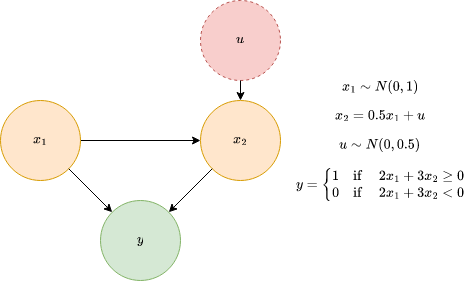
\includegraphics[width=0.8\linewidth]{images/toy_scm.png}
	\caption{A simple structural causal model}
	\label{fig:toy_scm}
\end{figure}

When incorporating a causal graph into the cost function, it is more appropriate to express the cost function as the cost of \textit{interventions} $\mathbf{a}=[a_1, a_2]^T$ with ordering $\mathbf{o}=[o_1, o_2]$, as opposed to cost of changing features $\mathbf{x}$ to $\mathbf{x}'$. The ordering dictates the order in which in the features are intervened upon, and the interventions dictate the size of the intervention. \todo[size=\small]{Add in worked example showing ordering matters in cost function.} The causal graph can be expressed as a weighted adjacency matrix $W$, where $W_{ij}$ is the marginal effect of intervening on $\mathbf{x}_i$ on $\mathbf{x}_j$. The cost of the interventions $\mathbf{a}$, given ordering $\mathbf{o}$ and weighted adjacency matrix $W$, is therefore the sum of a cost function over each individual intervention $\mathbf{a}_i$ (for example $c(\mathbf{a}_i) = \mathbf{a}_i^2$). The cost of the intervention can be expressed as follows, where $D$ is the number of features. 

\begin{equation}
	c(\mathbf{a}) = \sum_{i=1}^D c(\mathbf{a}_i)
\end{equation}

The post-intervention features $\mathbf{a}^*$ can be calculated as shown in Algorithm \ref{algo:causal_cost_function}.

\begin{algorithm}
	\caption{Intervention Evaluation Function}
	\begin{algorithmic}[1]
		\Function{EvalInterventions}{$\mathbf{a}, \mathbf{x}, \mathbf{o}, W$}
			\State \textbf{Input:} size of actions for each feature $\mathbf{a}$, original features $\mathbf{x}$, order of actions $\mathbf{o}$, adjacency matrix $W$
			\State \textbf{Output:} new features $\textbf{x}^*$
			\State $\textbf{x}^* \leftarrow \textbf{x}$
			\State $W \leftarrow W + I$ \Comment{where $I$ is the identity matrix}
			\State $\mathbf{s} \leftarrow \texttt{argsort}(\mathbf{o})$
			\For{$i$ in $\mathbf{s}$}\Comment{Loop through each feature in order of action}
				\State $\textbf{x}^* \leftarrow \textbf{x}^* + \mathbf{a}_i \times W[:,i]^{T}$ \Comment{Update for downstream effects}
			\EndFor
			\State \Return $\mathbf{x}^*$
		\EndFunction
	\end{algorithmic}
	\label{algo:causal_cost_function}
\end{algorithm}

\section{Generating recourse}

Using the new formulation of the cost function as the cost of interventions, we can also re-write the recourse generation problem, given a classifier $h$, original features $x$ and weighted adjacency matrix $W$. We denote the intervention evaluation as described in Algorithm \ref{algo:causal_cost_function} as \texttt{eval}. For negatively classified individuals, the task of recourse involves solving equation \ref{eq:recourse_gen_interventions}, where we minimise the cost of intervention subject to the new features $\mathbf{x}'$ leading to a positive classification (which corresponds to a classification score of greater than 0.5).

\begin{align} \label{eq:recourse_gen_interventions}
	\mathbf{a}', \mathbf{o}' = & \argmin_{\mathbf{a, o}} \sum_{i=1}^D c(\mathbf{a}_i) \\ \nonumber
	& \text{ s.t. } h(\texttt{eval}(\mathbf{a, x, o}, W)) \geq 0.5
\end{align}

As \texttt{eval} is a non-convex function, we cannot solve this constrained optimisation problem using convex optimisation. Instead, is converted into a unconstrained problem using Lagrange multipliers as shown in equation \ref{eq:lagrange_formulation}. This is solved using gradient descent, where at each iteration, a step is first taken to maximise $\lambda$ and then a step is then taken to minimise $\mathbf{a}$ and $\mathbf{o}$.

\begin{equation} \label{eq:lagrange_formulation}
	\min_{\mathbf{a, o}} \max_\lambda \sum_{i=1}^D c(\mathbf{a}_i) - \lambda (h(\texttt{eval}(\mathbf{a, x, o}, W))-0.5)
\end{equation}

This expression is possible to optimise using gradient descent when only optimising for $\mathbf{a}$, the function \texttt{eval} contains the line $S \leftarrow \texttt{argsort}(\mathbf{o})$, which is non-differentiable. Therefore, when optimising for the ordering $\mathbf{o}$, we must find an alternative to the \texttt{argsort} operator.

\subsection{Differentiable sorting}

The key point to make in this section is that technically, as long as a function is differentiable and maps from $f: \mathbb{R}^D \rightarrow \texttt{ordering}^D$, we should be able to take derivatives of $f$ and use gradient descent to find the value of the input to $f$ which minimises the objective defined in equation \ref{eq:lagrange_formulation}. The smoother the function is in its mapping from a vector of real numbers to the ordering (i.e., vectors close to each other map to similar orderings), the fewer local minima it should have, making optimisation easier.

\section{Learning from revealed preferences}

\todo[size=\small]{To re-write below this point.}

We do not observe the cost function itself, but one way to approximate it is to \textit{learn from revealed preferences} (see section \ref{section:revealed_pref_lit}). We propose that each individual who is negatively classified is presented with $N$ pairs of recourse options $((\mathbf{a}_n^1, \mathbf{o}_n^1),(\mathbf{a}_n^2, \mathbf{o}_n^2))$. Each of the recourse options corresponds to a list of actions and associated orderings. The individuals, for each of the $N$ pairs of recourse options, then select which one is preferable. \todo[size=\small]{Need to rephrase actions as the total action (even if you get part of it for 'free'.}

If, for a single pair of recourse options $((\mathbf{a}_n^1, \mathbf{o}_n^1),(\mathbf{a}_n^2, \mathbf{o}_n^2))$, option 1 is selected, then we assume that $\sum_{i=1}^D c(\mathbf{a}^1_{ni}) \leq \sum_{i=1}^D c(\mathbf{a}^2_{ni})$. If option 2 is selected, we assume the opposite, that $\sum_{i=1}^D c(\mathbf{a}^1_{ni}) > \sum_{i=1}^D c(\mathbf{a}^2_{ni})$. The responses to the pairs of recourse options presented (the pairwise comparisons) reveal information about the individuals' preferences over recourse options, i.e., their cost functions over individual features. \todo[size=\small]{User preference over cost functions involves knowledge of the causal graph, should this then be optimised for in learning from revealed preferences.)}

Once a cost function is learned, we need to solve the optimisation problem mentioned in equation \ref{eq:lagrange_formulation} to generate the recourse $(\mathbf{a}', \mathbf{o}')$.

\subsection{Weighted Squared Costs}

Let the individual cost function take the form $c(\mathbf{a}, \beta) = \sum_{i=1}^D \beta_i \mathbf{a}^2_i$, where $\beta \in \mathbb{R}^D$ is a vector which expresses the mutability of each feature $i$. To learn the cost function, we need to learn $\beta$.

Given a fixed weighted adjacency matrix $W$,\todo[size=\small]{Seems much more efficient to assume a fixed ordering} we can denote the response of the $n$th paired comparison as follows.

\begin{equation} \label{eq:paired_response}
	y_{n} = \begin{cases}
		-1 & \text{if } \sum_{i=1}^D c(\mathbf{a}^1_{ni}) \leq \sum_{i=1}^D c(\mathbf{a}^2_{ni}) \\
		+1 & \text{if }  \sum_{i=1}^D c(\mathbf{a}^1_{ni}) > \sum_{i=1}^D c(\mathbf{a}^2_{ni}) \\
	\end{cases}
\end{equation}

We optimise for when $y_n$ and $\hat{y}_n$ (the predicted value of $y_n$, using our initial guess of $\beta$) are similar. A optimisation to do this is shown below, where there are $K$ individuals and $N$ pairwise comparisons and $\ell(y, \hat{y}) = \max[0, 1-y\hat{y}]$ represents the hinge loss.

\begin{equation}
	\argmin_\beta = \frac{1}{KN} \sum_{k=1}^K \sum_{n=1}^N \ell (y_{kn}, \hat{y}_{kn}(\beta)) + \underbrace{\lambda ||\beta||_2}_{\text{L2 regularisation}}
\end{equation}

This is an unconstrained optimised problem that can be optimised via gradient descent. However, operation in equation \ref{eq:paired_response} is non, differentiable, so instead it is approximated with the below expression, which fits $\hat{y}_n$ into [-1,1] where $\lambda$ is a hyperparameter regularising for 'confidence' of the predictions.

\begin{equation}
	\hat{y}_n = \tanh \Bigg(\lambda \Big(\sum_{i=1}^D c(\mathbf{a}^1_{ni}) - \sum_{i=1}^D c(\mathbf{a}^2_{ni})\Big)\Bigg)
\end{equation}


\section{Mahalanobis distance}

The Mahalanobis distance between the vector $\mathbf{x}$ and the vector $\mathbf{y}$ is defined in equation \ref{eq:mahalanbobis_distance}, where $M$ is a positive semi-definite matrix.

\begin{equation} \label{eq:mahalanbobis_distance}
	||\mathbf{x-y}||_{\mathbf{M}} = \sqrt{(\mathbf{x-y})^T\mathbf{M}^{-1}(\mathbf{x-y})}
\end{equation}

The matrix $\mathbf{M}$ captures different relationships between the features within $\mathbf{x}$ and $\mathbf{y}$ in the off-diagonal elements of $\mathbf{M}$. If $\mathbf{M}$ is set to the identity matrix, then the Mahalanobis distance then becomes equal to the Euclidean distance between $\mathbf{x}$ and $\mathbf{y}$. \\

\subsection{Learning the Mahalanobis distance}

In order to use the Mahalanobis distance as a cost function, we must learn the matrix $\mathbf{M}$. In this set-up, each individual $k$ with original features $\mathbf{x}_k$ is presented with $N$ recourse options $(\mathbf{x}_{kn}^a, \mathbf{x}_{kn}^b)$. The response $y_{kn}$ is defined in equation \ref{eq:response_definition}, where $c^G_k$ represents the ground truth cost function of individual $k$.

\begin{equation} \label{eq:response_definition}
	y_{kn} = \begin{cases}
		-1 & \text{if } c^G_k(\mathbf{x}_{kn}, \mathbf{x}^a_{kn}) \leq c^G_k(\mathbf{x}_{kn}, \mathbf{x}^b_{kn}) \\
		+1 & \text{if } c^G_k(\mathbf{x}_{kn}, \mathbf{x}^a_{kn}) > c^G_k(\mathbf{x}_{kn}, \mathbf{x}^b_{kn}) \\
	\end{cases}
\end{equation}

To optimise for $\textbf{M}$, we compare the squared Mahalanobis distances between $\textbf{x}_k$ and $\textbf{x}^a_{kn}$ and between $\textbf{x}_k$ and $\textbf{x}^b_{kn}$. The optimisation problem to learn $\textbf{M}$ is shown in equation \ref{eq:mahalanobis_non_convex}, where $\ell$ represents either the hinge or logistic loss function. The optimisation is an adaptation of the optimisation problem presented in \textcite{canalOneAllSimultaneous2022}.

[\textbf{TO ADD EXPLANATION ON WHY THIS IS A GOOD OPTIMISATION}]

\begin{align} \label{eq:mahalanobis_non_convex}
	\min_{\mathbf{M}} & \frac{1}{KN} \sum_{k=1}^K \sum_{n=1}^N \ell \bigg( y_{kn} \big(|| \mathbf{x}_k - \mathbf{x}_{kn}^a ||^2_{\mathbf{M}} - || \mathbf{x}_k - \mathbf{x}_{kn}^b ||^2_{\mathbf{M}} \big) \bigg) \\	
	\text{s.t. } & \mathbf{M} \succeq 0, \nonumber
\end{align}

\section{Convex layers}

To look into convex neural networks using \href{https://github.com/cvxgrp/cvxpylayers}{\texttt{cvxpylayers}}, which is based on \textcite{agrawalDifferentiableConvexOptimization2019}.
